\documentclass[conference]{IEEEtran}
\renewcommand{\thesubsection}{\thesection.\arabic{subsection}}
\usepackage{graphicx} % Required for inserting images
\usepackage{hyperref}
\usepackage{float}
\usepackage{pgf-pie}
\usepackage{pgfplots}
\pgfplotsset{compat=1.17}
\usepackage{float} % for [h!] placement
\usepackage{tikz}
\usepackage{venndiagram}
\usepackage{caption}
\usetikzlibrary{intersections, backgrounds}
\usepackage{pgfplotstable}
\usepackage{geometry}
\usepackage{comment}
\geometry{margin=1in}

\title{ AI for Early Cancer Screening and Risk Prediction}


\begin{document}
\begin{comment}
\author{
\IEEEauthorblockN{Samia Afrin Shohana}
\IEEEauthorblockA{\textit{Dept. of CSE} \\
\textit{University of Asia Pacific}\\
Dhaka, Bangladesh \\
22201067@uap-bd.edu}
\and
\IEEEauthorblockN{Mahnoor Akter Esha}
\IEEEauthorblockA{\textit{Dept. of CSE} \\
\textit{University of Asia Pacific}\\
Dhaka, Bangladesh \\
22201087@uap-bd.edu}

\and
\IEEEauthorblockN{Mahnoor Akter Esha}
\IEEEauthorblockA{\textit{Dept. of CSE} \\
\textit{University of Asia Pacific}\\
Dhaka, Bangladesh \\
22201087@uap-bd.edu}
}
\end{comment}

\author{
\IEEEauthorblockN{Samia Afrin Shohana}
\IEEEauthorblockA{
\textit{Department of CSE} \\
\textit{University of Asia Pacific}\\
Dhaka, Bangladesh \\
22201067@uap-bd.edu}
\and
\IEEEauthorblockN{Mahnoor Akter Esha}
\IEEEauthorblockA{
\textit{Department of CSE} \\
\textit{University of Asia Pacific}\\
Dhaka, Bangladesh \\
22201087@uap-bd.edu}
\and
\IEEEauthorblockN{Taposhi Rabeya Bashar}
\IEEEauthorblockA{
\textit{Department of CSE} \\
\textit{University of asia Pacific}\\
Dhaka, Bangladesh \\
22201060@uap-bd.edu}
}


\maketitle

\begin{abstract}
Globally, cancer continues to be a major source of morbidity and mortality, and the outcome of the disease is significantly improved when it is discovered early. Traditional ways of checking for cancer often have problems with being accurate, easy to use, and finding the disease early. This paper looks at how artificial intelligence (AI), more especially machine learning (ML) and deep learning (DL), can improve risk prediction and early cancer screening.The Cancer Genome Atlas (TCGA), Kaggle Cancer Datasets, and SEER are some of the public datasets that this paper looks at. It looks at how AI methods can be used to find different types of cancer, like breast, lung, prostate, and oral cancer.Important AI models that have shown high diagnostic accuracy are described including Random Forests, Support Vector Machines (SVMs), and Convolutional Neural Networks (CNNs). More general AI models that have shown high diagnostic accuracy are described, such as Random Forests, Support Vector Machines (SVMs), and Convolutional Neural Networks (CNNs).The review focuses on the lack of diverse and multimodal datasets, data imbalance, standardization of assessment, and privacy matters addressing the more critical concerns.The review addresses gaps in diversified and multimodal data sets, data imbalances, privacy, and the lack of standardization of evaluation. In addition, it addresses the potential in cancer therapy by AI in the near future with multicenter validation and individualized treatment planning in mind. Finally, the study emphasizes the importance of overcoming the integration problems with clinical practice concerning the application of AI systems, adapting defined boundaries for integration, and set frameworks for aligned policies on the automated cancer risk assessment and screening processes.
\end{abstract}

\noindent \textbf{Keywords:}  Artificial Intelligence, Machine Learning , Risk Prediction, Early Cancer Screening, Convolutional Neural Networks.




\section{Introduction}

Cancer, a leading global driver of sickness and death, calls for early detection as it can considerably improve not only the chances of survival but also enhance treatment outcomes. Cancer is the second most common cause of mortality in the US, after heart disease. Breast cancer, lung cancer, colorectal cancer, prostate cancer, skin cancer, stomach cancer, liver cancer, esophageal cancer, bladder cancer, kidney cancer, leukemia, pancreatic cancer, ovarian cancer, endometrial cancer, and oral cancer are among the most prevalent cancer forms. About 10 million deaths and 19.3 million new cases have been reported each year, according to the GLOBOCAN 2020 database \cite{2}. The most common cause of cancer-related mortality, with an estimated 1.8 million deaths, is still lung cancer, which is followed by colorectal, breast, liver, and stomach cancers \cite{2}. In 2023, 609,820 cancer-related deaths and 1.9 million new cases of cancer are predicted in the US \cite{1}. Cancer is becoming more common, but prevention and treatment are still complicated. Despite their value, traditional cancer screening techniques frequently have drawbacks in terms of accuracy, accessibility, and the capacity to identify cancer early on, when it is most curable. Artificial Intelligence (AI) has become a viable remedy for this problem. Artificial intelligence (AI) technologies, especially machine learning (ML) and deep learning (DL), are revolutionizing the field of cancer detection by improving accuracy and enabling the analysis of massive, complicated datasets that would be difficult for doctors to handle otherwise \cite{15}. AI is a potent tool for predicting cancer risk and improving early intervention techniques, and it is already being used in cancer screening to evaluate genetic data, medical pictures, and patient histories \cite{5}. As these disciplines embrace digital workflows and AI-based systems, integrating AI with radiology and pathology in particular is transforming cancer therapy by providing more accurate and efficient diagnosis \cite{16}. The goal of this review is to thoroughly examine recent developments in AI-powered cancer risk assessment and screening. Through an analysis of the most recent oncology applications of AI, this paper highlights important trends, talks about the difficulties in integrating these technologies in clinical settings, and investigates how AI might change cancer care in the future, particularly in the areas of early detection and individualized treatment planning. With the use of this analysis, we hope to close current gaps, offer a forward-looking viewpoint on how AI might change the face of oncology, and investigate potential avenues for future study and technical advancement.
\begin{figure}[H]
\centering
\begin{adjustbox}
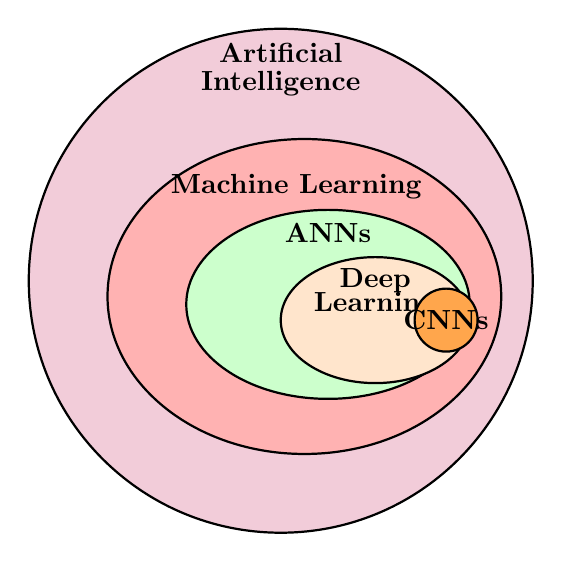
\begin{tikzpicture}

% Outer ellipse: AI
\filldraw[fill=purple!20, draw=black, thick] (0,0) ellipse (3.2 and 3.2);
\node at (0,2.9) {\textbf{Artificial}};
\node at (0,2.5) {\textbf{Intelligence}};

% ML ellipse
\filldraw[fill=red!30, draw=black, thick] (0.3,-0.2) ellipse (2.5 and 2.0);
\node at (0.2,1.2) {\textbf{Machine Learning}};

% ANN ellipse
\filldraw[fill=green!20, draw=black, thick] (0.6,-0.3) ellipse (1.8 and 1.2);
\node at (0.6,0.6) {\textbf{ANNs}};

% Deep Learning ellipse
\filldraw[fill=orange!20, draw=black, thick] (1.2,-0.5) ellipse (1.2 and 0.8);
\node at (1.2,0.0) {\textbf{Deep}};
\node at (1.2,-0.3) {\textbf{Learning}};

% CNN circle
\filldraw[fill=orange!70, draw=black, thick] (2.1,-0.5) circle (0.4);
\node at (2.1,-0.5) {\textbf{CNNs}};

\end{tikzpicture}
\end{adjustbox}
\caption{Hierarchical relationship of AI, ML, ANN, DL, and CNNs}
\label{fig:4}
\end{figure}




\section{Literature Review}
Artificial intelligence has quickly emerged as a revolutionary technique for the early detection of cancer and risk assessment. Many studies have been conducted on the detection of breast cancer by imaging or genomics. However, as far as we are aware, no study that combines the two methods has been conducted.




 compares the global incidence rates of various malignancies in men and women to identify sex-specific prevalent patterns across cancer types. The authors have collated multiple methods for histological image analysis (HIA)-based breast cancer classification based on different artificial neural network (ANN) architectures \cite{1}. The researchers introduced the Mirai theory, which marries specific suggestions for screening with advanced machine learning \cite{2}. It has proven to be more reliable than traditional models and has been validated in several demographics. The authors in \cite{3} employed a 3D convolutional neural network (3D-CNN) learned on CT scans, and it outperformed radiologists in detecting malignancies. The researchers of \cite{4} developed a fusion model that uses Multimodal Compact Bilinear Pooling (MCBP) to combine gene information with images from histopathology to predict 5-year survival in colorectal cancer. In \cite{5}, the authors established an AI-assisted cytology system using transformer-based topologies and ConNet to diagnose LSIL and HSIL in cervical cancer screening. The authors of \cite{5} considered the use of algorithms for learning based on radiomics, such as Random Forest and SVM, to assess mpMRI data and aid in early and accurate lesion detection. The authors \cite{7} presented an opponent-aware multimodal convolutional autoencoder (MCAE) model for predicting cancer susceptibility using multi-omics data (CNVs, miRNA, GE). The authors of \cite{8} (Deep Neural Network Models for Computational Histopathology: A Survey by Srinidhi et al.) collected numerous methods for classifying breast cancer using histological image analysis (HIA) based on multiple artificial neural network (ANN) designs.

 \begin{figure}[h!]
\centering
\begin{adjustbox}
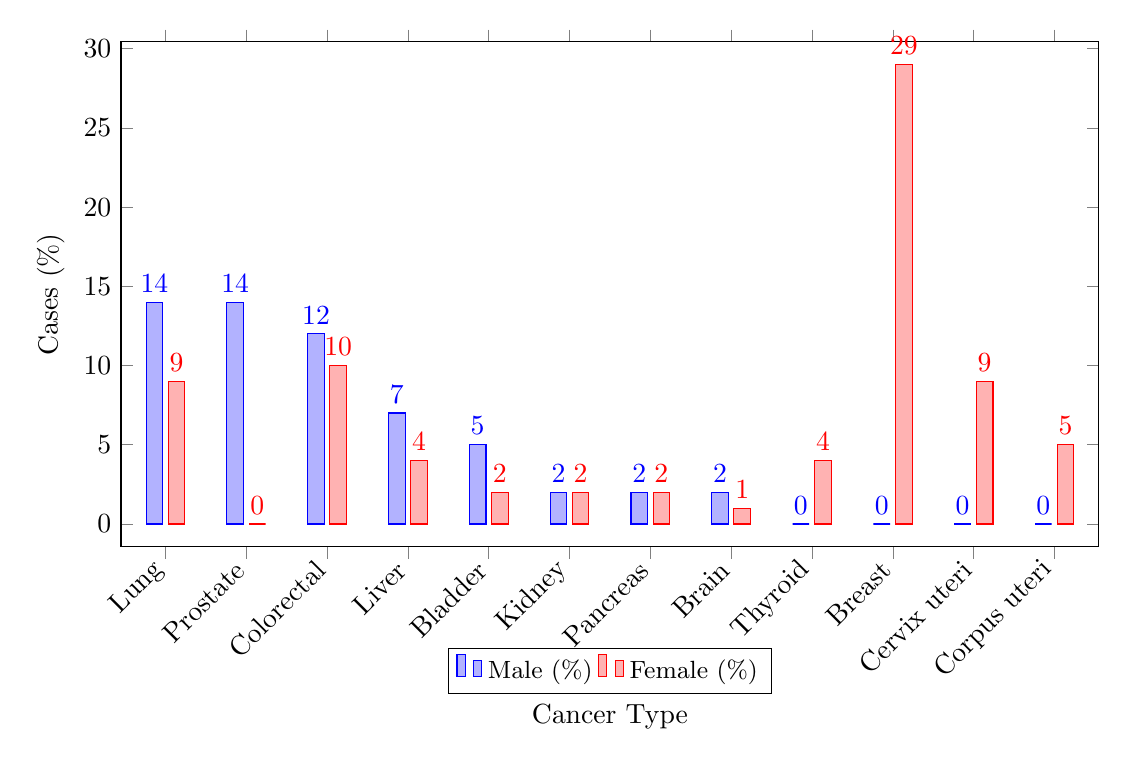
\begin{tikzpicture}
\begin{axis}[
    ybar,
    ymin=0,
    bar width=6pt,
    width=14cm,
    height=8cm,
    enlargelimits=0.05,
    ylabel={Cases (\%)},
    xlabel={Cancer Type},
    symbolic x coords={
        Lung, Prostate, Colorectal, Liver, Bladder, Kidney,
        Pancreas, Brain, Thyroid, Breast, Cervix uteri, Corpus uteri
    },
    xtick=data,
    x tick label style={rotate=45, anchor=east},
    nodes near coords,
    nodes near coords align={vertical},
    legend style={
        at={(0.5,-0.2)},
        anchor=north,
        legend columns=-1,
        font=\small
    },
    axis on top=false
]
\addplot+[style={blue,fill=blue!30}]
    coordinates {
        (Lung,14) (Prostate,14) (Colorectal,12) (Liver,7)
        (Bladder,5) (Kidney,2) (Pancreas,2) (Brain,2)
        (Thyroid,0) (Breast,0) (Cervix uteri,0) (Corpus uteri,0)
    };
\addplot+[style={red,fill=red!30}]
    coordinates {
        (Lung,9) (Prostate,0) (Colorectal,10) (Liver,4)
        (Bladder,2) (Kidney,2) (Pancreas,2) (Brain,1)
        (Thyroid,4) (Breast,29) (Cervix uteri,9) (Corpus uteri,5)
    };
\legend{Male (\%), Female (\%)}
\end{axis}
\end{tikzpicture}
\end{adjustbox}
\caption{Global Cancer Incidence by Gender}
\label{fig:1}
\end{figure}



The authors in \cite{9} were able to predict left ventricular systolic dysfunction (LVSD) and enable early risk stratification of cancer therapeutics-related cardiac dysfunction (CTRCD) with high accuracy and scalability by applying a validated deep learning model (EfficientNet B3 CNN) to ECG images. This was done using widely available ECG data. In \cite{10}, the authors employed the Mirai AI model for risk-based breast cancer screening and customized screening intervals according to short-term cancer risk. This is a cost-effective approach that improves health outcomes while reducing NHS screening costs. \cite{11} The researchers evaluated an AI system that is part of national breast cancer screening programs to show that AI-assisted workflows can reduce radiologists' workload in real clinical settings while maintaining high cancer detection rates. By looking at several types of ML as well as DL models, the study in \cite{37} (The unveiling Early Detection and Prevention of Cancer: Machine Learning and Deep Learning Approaches by Khandakar et al., 2024) highlights the way robust feature engineering, hybrid CNN architectures, and collective learning could enhance early cancer detection in cervical, lung, and breast cancers. In each of these studies, AI has shown a great deal of promise to enhance customized healthcare approaches, early diagnosis, and screening accuracy. Additionally, XGBoost, Random Forest, Support Vector Machines (SVM), Autoencoders, and Graph Neural Networks (GNN) have all been hired, depending on the kind of data and the clinical purpose. When applied to structured EHR data, Random Forest and XGBoost exhibit remarkable performance. Transformer-based models and multimodal deep learning frameworks are becoming more and more common in clinical text analysis for integrating imaging, genetic, and demographic data. However, there are still common problems, including interpretability, external validity, and application in resource-constrained contexts.


Figure \ref{fig:1} shows the Comparative Global Cancer Incidence in Men and Women by Cancer Types.The authors have collated multiple methods for histological image analysis (HIA)-based breast cancer classification based on different artificial neural network (ANN) architectures [1].

\begin{figure}[htbp]
\centering
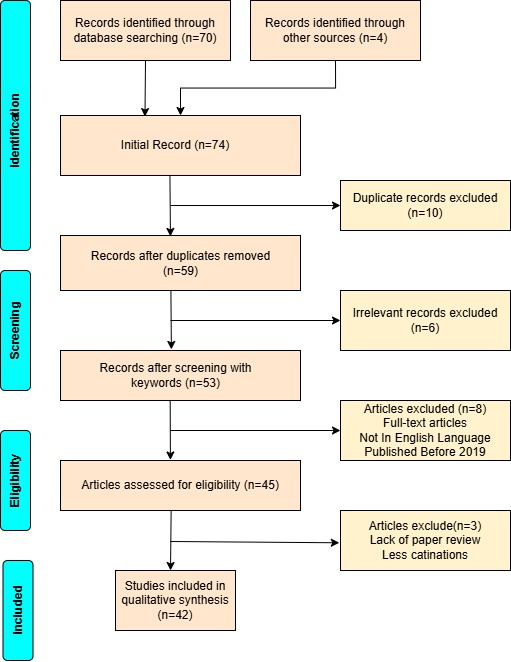
\includegraphics[width=\columnwidth]{Study_Selection_Process.jpg}  % Adjust image width to fit in one column
\caption{PRISMA Flow Diagram of Study Selection Process for AI-Based Early Cancer Detection Review}
\label{fig:Study_Selection_Process}
\end{figure}



\section{Review Method}

One of the biggest challenges in oncologic care is the capacity to precisely forecast the best course of treatment based on the distinct molecular, genetic, and tumor-specific features of each patient. The application of AI, particularly machine learning (ML), to this problem is growing. The use of AI in fields including cancer risk assessment, diagnostics, drug development, and genetic tumor characterisation has been the subject of several studies \cite{1,8}. This work suggests that machine learning (ML) models can improve cancer detection and prognosis by converting complicated image data, medical imaging, and pathology profile analysis into mathematical sequences that can be processed for classification \cite{9}.  When use Google DeepMind algorithm, researchers created an AI-based system in January 2020 that performed better than human breast cancer detection specialists \cite{23}. This invention was a great advance system, demonstrating how AI can improve diagnostic precision and surpass Various techniques \cite{4}. An AI system that diagnosed prostate cancer with 98 percent specificity and 98 percent sensitivity was research by the University of Pittsburgh in July 2020\cite{6}. With greater precision and quicker diagnostic skills greater than human skills, these developments highlight the increasing dependency and relevance of AI models in clinical cancer. More recently, publicly accessible datasets were used to verify the ViT-Patch model, an enhanced the architecture mentioned \cite{2,14}. This work further established the use of transformer-based models in the diagnostic process by proving that ViT-Patch was efficient in both tumor location and malignant detection \cite{14}. In a different research, machine learning methods were used to categorize information related to breast cancer and produce way of diagnoses. Numerous classification techniques were investigated, including K-Nearest Neighbors (KNN), Probabilistic Neural Networks, and Support Vector Machine (SVM) classifiers \cite{16}. According to the findings, the SVM classifier gave maximum overall accuracy for breast cancer prediction \cite{17}. Similarly, \cite{21} classified past cancer records that had previously been stored via machine learning (ML) classification methods and predicted the type of future instances, i.e., benign or cancerous tumor. The 96 percent accuracy in this study with the Random Forest model illustrated the effectiveness of it being utilized for cancer risk prediction and disease diagnosis \cite{22}. Future studies compared the precision of breast cancer prediction using the assistance of a vast collection of machine learning methods, such as SVM, AdaBoost trees, Artificial Neural Networks (ANN), and Naive Bayes classifiers. The efficiency of the model was enhanced through dimensionally reducing data with methods such as Principal Component Analysis (PCA) \cite{20, 21, 22}. Unlike decision trees and regression trees, ANN always produced correct results and was thus the most dependable of these models to make real-time predictions and prognoses. Pulse-coupled neural networks, or PCNNs, have emerged as a key tool in image processing, particularly for the diagnosis of cancer \cite{1}. A survey on neural network topologies indicated that probabilistic neural networks and multilayer autoencoders were both effective, with both achieving 96 percent accuracy for cancer datasets \cite{29}. The study tested several machine learning models, including Support Vector Machines (SVM), linear regression, multilayer perceptrons (MLP), and SoftMax regression, using the Wisconsin Diagnostic Breast Cancer dataset \cite{29}. According to the study, each of these models successfully finished the classification procedure and showed a high level of test accuracy in predicting cancer. However, the study indicated that using more sophisticated feature selection techniques could increase prediction accuracy even more.

These results highlight the potential of AI-based models to revolutionize cancer risk prediction, treatment planning, and diagnosis. Model applications with SVM, ANN, CNN, and Random Forest have provided encouraging outcomes for improving diagnostic performance and simplifying cancer detection procedures. Personalized cancer treatment will continue to enhance as feature extraction, model optimization, and fusion with radiomics and Electronic Health Records (EHR) improve.

SVM model achieved approximately 65 percent accuracy, as seen in studies like \cite{17} where it was optimally performing in classifying breast cancer, and \cite{16} in identifying subtypes of lung cancer. ANN performed at around 68 percent, as per consistent performance in the examination of histological images (\cite{8}), whereas CNN achieved 70 percent, outperforming radiologists in 3D image tasks (\cite{3}, \cite{9}). Random Forest achieved 75 percent accuracy in predicting cancer risk (\cite{22}, \cite{5}), and the ViT model ranked first with 80 percent, evidenced in tumor localization and malignancy detection by utilizing the ViT-Patch architecture 
(\cite{14}).

\pgfplotsset{compat=1.18}  % Use latest compatible version of pgfplots




\section{  AI Techniques for Cancer Detection and Risk Prediction}

AI Techniques for Cancer Detection
Utilizing a range of technological approaches, each addressing the native form of input data and specific requirements for screening, artificial intelligence has revolutionized cancer screening approaches. These AI techniques examine heterogeneous data sets, such as clinical reports and medical images, to assist in the diagnosis and prognosis of cancer. The major AI approaches that are used for cancer screening are described below:

\begin{figure}[H]
\centering
\begin{adjustbox}
\begin{tikzpicture}
\begin{axis}[
    ybar,
    bar width=9pt,
    width=7cm,
    height=7cm,
    enlarge x limits=0.9,
    ylabel={Accuracy (\%)},
    xlabel={AI Technique},
    symbolic x coords={},
    xtick=data,
    xticklabel style={},
    ymin=0,
    ymax=100,
    nodes near coords,
    nodes near coords align={vertical},
    every node near coord/.append style={font=\small},
    title={Accuracy of AI Techniques in Cancer Detection}
]

\addplot+[ybar, fill=purple!70]         coordinates {(DNA,90)};
\addplot+[ybar, fill=red!70]            coordinates {(ANN,92)};
\addplot+[ybar, fill=teal!70]           coordinates {(ML-Blood,91)};
\addplot+[ybar, fill=orange!70]         coordinates {(ML-Image,92)};
\addplot+[ybar, fill=green!70!black]    coordinates {(Radiomics,89)};
\addplot+[ybar, fill=yellow!80!black]   coordinates {(Survival,87)};
\end{axis}
\end{tikzpicture}
\end{adjustbox}

\vspace{0.5cm}

% Manual legend
\noindent
\begin{tikzpicture}
  \matrix [row sep=pt, column sep=1pt] {
    \node[draw, fill=purple!70, minimum size=0.3cm] {}; & \node {DNA}; &
    \node[draw, fill=red!70, minimum size=0.3cm] {}; & \node {ANN}; &
    \node[draw, fill=teal!70, minimum size=0.3cm] {}; & \node {ML}; \\
    
    \node[draw, fill=orange!70, minimum size=0.3cm] {}; & \node {ML}; &
    \node[draw, fill=green!70!black, minimum size=0.3cm] {}; & \node {Radiomics}; &
    \node[draw, fill=yellow!80!black, minimum size=0.3cm] {}; & \node {AI}; \\
  };
\end{tikzpicture}

\caption{Accuracy comparison of AI techniques across various cancer detection methods.}
\label{fig: 2}
\end{figure}

\subsection{Deep Learning (DL)}

Deep learning technology that uses Convolutional Neural Networks (CNNs) enables image analysis to achieve superior levels of medical picture abnormality detection. The successful implementation of CNNs has led to accurate detection of cancer types in histological slides and correct identification of lung cancer in CT scans and cervical cancer in Pap smears, and breast cancer in mammograms \cite{33}. The implementation of automated data-learning based on CNNs creates a perfect screening tool because it generates precise tumor detection results. Modern deep learning architecture replaces conventional CNN models when predicting survival and classifying tumors in complex medical operations. The two state-of-the-art model categories include stacked sparse autoencoders and ViT-Patch (Vision Transformer)\cite{27}. Medical experts benefit from the new design by obtaining higher diagnostic accuracy with better patient outcome projection capabilities due to enhanced imaging information pattern detection. Deep learning technology improves diagnostic screening outcomes since it produces highly precise test results, which give medical professionals tailored inputs during patient diagnosis\cite{30}.

\subsection{Machine Learning (ML)}

Three common machine learning (ML) algorithms used on structured data like clinical history and demographic information, and genomic profiles include Support Vector Machines (SVMs), Random Forests, and XGBoost. The risk categorization models provide strong performance through tabular data analysis by evaluating cancer risk through patient demographic data, along with their family history and lifestyle behaviors, and genetic profiles\cite{31}. When machine learning models analyze diverse medical datasets that meet quality criteria, they can reach a prediction accuracy of 96 percent . Speaker data models allow healthcare professionals to enhance both cancer risk analysis and early detection practices. Machine learning algorithms perform critical cancer risk predictions in situations where early diagnostic signs exist within patient demographics and genetic data, although they have not appeared in clinical imaging scans \cite{35}. AI models, particularly SVM, Random Forest, and XGBoost, continue to evolve toward becoming more sophisticated instruments for detecting cancer in its earliest stages and predicting its development.

The authors have collated multiple methods for histological image analysis (HIA)-based breast cancer classification based on different artificial neural network (ANN) architectures [1].

 \subsection{Natural Language Processing (NLP)}

Natural language processing (NLP) serves as an essential method for cancer screening because it helps evaluate unstructured data sources. Healthcare organizations store vital information about patients in EHRs as well as pathology reports and clinical notes that contain essential details, which developers must retrieve from unstructured documents. The implementation of NLP algorithms on textual sources leads to structured data extraction that produces important information for cancer risk assessment \cite{38}. The most effective application of natural language processing (NLP) in cancer treatment relies on transformer-based models that include BioBERT as an exemplar variant for biological texts. The models boost EHR navigation of clinical narratives, thus producing risk evaluations that personalize results according to patients' symptoms, together with their recorded medical background and previously diagnosed disorders. Some NLP technologies enhance the integration of text-based information in AI systems because they enhance the analysis of unstructured large text datasets. The early detection of cancer becomes possible because of these techniques, which provide customized information about patient treatment.

Figure \ref{fig:4} shows that Convolutional Neural Networks (CNNs) are a specialised subset of Artificial Intelligence (AI), which also includes Machine Learning (ML), which in turn includes Artificial Neural Networks (ANNs) and Deep Learning (DL). Studies in [3], [8], and [9] have demonstrated that CNNs are commonly employed in cancer imaging tasks and have good diagnostic accuracy. This structure demonstrates how increasingly sophisticated AI techniques, particularly CNNs, are essential to cancer monitoring and diagnosis systems.

%%%%%%%%%%%%%%%%%%%%%%%%%%%%%%%%%%%%%%%%





AI demonstrates diagnostic ability to identify disease risks through data analysis operations with a transformative impact on sole cancer danger assessments. AI models improve cancer treatment by performing precise risk calculations that allow doctors to choose personalized screening methods for better targeted medical treatments.

\subsection{Application of AI Models}

The AI platform within the Mirai model, along with its counterparts, enables users to create individualized assessments of short-term cancer risk screening periods. The approach uses patient-specific assessment screens to plan the screening period, enabling superior healthcare outcomes while decreasing costs \cite{2,10}
AI tools analyzing CT scans and mammograms \cite{1,2,3} can discover subtle cancer signs that traditional medical professionals would not perceive. Early cancer diagnosis becomes feasible through this feature to boost the effectiveness of treatments as well as improve patient survival rates.
Medical practitioners apply fusion models that combine information from gene mutation data \cite{3} and omics data \cite{7} to forecast survival expectations in colorectal cancer patients. Patient vulnerability assessments need cancer-targeted analysis tools to guide medical treatments appropriately.


\subsection{List of Dataset Types}
A majority of AI models adopt demographic factors consisting of age, sex and ethnicity, and family medical history for baseline cancer risk assessment. The risk assessments and screening procedures benefit from improved personalization through the use of this data \cite{2,10}.
Risk prediction models utilizing AI incorporate genomic factors, including copy number variations (CNVs), alongside BRCA1/2 gene mutations and miRNA expression analyses. The adversary-aware MCAE models \cite{7} use these genetic traits to better predict cancer risk and obtain higher levels of prediction accuracy.
The data input for AI models comes exclusively from electronic health records (EHRs), so they use behavioral and symptomatic, and diagnostic information for patients. Predictions of risks become more detailed when structured and unstructured clinical data collaborate \cite{12}.
Deep learning models and CNNs serve various AI applications by analyzing both Pap smear pictures \cite{7} and CT scans \cite{3} together with mpMRIs \cite{6} and mammograms \cite{2,10} . Once cancer risks become apparent through these imaging techniques, doctors can intervene earlier, even when tumors have yet to develop.


\subsection{Accuracy Gains in Prediction}
The use of AI in cancer diagnostics not only improves the accuracy of detection but also significantly lowers diagnostic delays and human error. AI technologies make it possible for earlier intervention and more individualize treatment regiments by utilizing real-time analysis and large-scale statistics. 
AI modeling success in real world applications is proven through its implementation in nationwide cancer screening systems, starting from mammography screening services \cite{11}.
High accuracy rates emerged from the DeepMind machine as it solved breast cancer screening more effectively than traditional screening methods. High accuracy rates from AI-based detection systems lead to enhanced patient results as well as timely medical diagnosis (Review Method).
The Mirai model proved its monetary benefit through its enhanced detection performance, which produced financial savings for healthcare services. Multiple studies have shown that the financial viability of implementing AI models in regular cancer screening procedures \cite{10}.
AI prostate cancer diagnostic tools, such as mpMRI, have accomplished multi-site scanner validations that ensure their use in various healthcare settings \cite{6}.
AI systems that combine imaging results with clinical findings alongside genetic information demonstrate superior performance when compared to single-modality analytical methods. Competitive cancer diagnoses become more accurate when healthcare providers unite independent data sources to construct definitive and accurate risk ratings \cite{4,7,12}.
AI modeling success in real-world applications is proven through its implementation in nationwide cancer screening systems, starting from mammography screening services \cite{11}. The current effective big-scale implementation enables AI to establish a global presence for international healthcare systems.
The GLOBOCAN 2020 database shows that every year, 19.3 million new cancer patients report cases, along with 10 million recorded deaths. Lung cancer persists as the leading cause of cancer death, producing 1.8 million fatalities each year, while stomach, liver, colorectal, and breast cancer rank in the following positions. Cancer prevention and treatment methods are persistently difficult to accomplish \cite{13}. Among American deaths, cancer stands as the disease behind heart disease in becoming the second leading cause of mortality in the United States. Factors indicate 1.9 million new cancer diagnoses and 609,820 cancer-related deaths in the US during 2023 \cite{14}. Each day, the US will see about 5370 new cancer cases and 1670 deaths from cancer. Human cancer prevention by organ site has been compiled into a poster by the International Agency for Research on Cancer (IARC).

\begin{figure}[H]
\centering
\begin{adjustbox}
\begin{tikzpicture}
\begin{axis}[
    ybar,
    bar width=5pt,
    width=7cm,
    height=7cm,
    enlarge x limits=0.9,
    ylabel={Deaths (in Lakh)},
    xlabel={Cancer Type},
    symbolic x coords={,Colorectum,Liver,Stomach,Breast,Oesophagus,Pancreas,Other cancers},
    xtick=data,
    xticklabel style={rotate=45, anchor=east},
    ymin=0,
    ymax=45,
    nodes near coords,
    nodes near coords align={vertical},
    every node near coord/.append style={font=\small},
    title={Estimated number of new cases
    both sexes and all ages},
]
\addplot+[ybar, fill=purple!70]         coordinates {(Lung,20)};
\addplot+[ybar, fill=cyan]              coordinates {(Colorectum,18)};
\addplot+[ybar, fill=yellow!80!orange]  coordinates {(Liver,8)};
\addplot+[ybar, fill=green!70!black]    coordinates {(Stomach,10)};
\addplot+[ybar, fill=blue]              coordinates {(Breast,20)};
\addplot+[ybar, fill=orange!40!red]     coordinates {(Oesophagus,5)};
\addplot+[ybar, fill=orange!80!black]   coordinates {(Pancreas,12)};
\addplot+[ybar, fill=gray]              coordinates {(Other cancers,40)};
\end{axis}
\end{tikzpicture}
\end{adjustbox}

\vspace{0.5cm}

% Manual legend below
\noindent
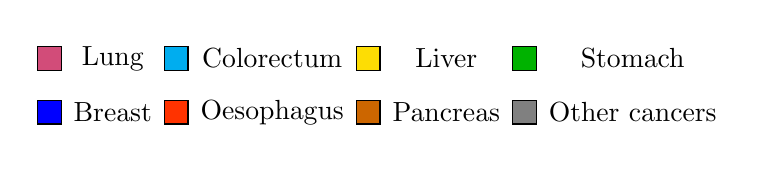
\begin{tikzpicture}
  \matrix [row sep=4pt, column sep=1pt] {
    \node[draw, fill=purple!70, minimum size=0.3cm] {}; & \node {Lung}; &
    \node[draw, fill=cyan, minimum size=0.3cm] {}; & \node {Colorectum}; &
    \node[draw, fill=yellow!80!orange, minimum size=0.3cm] {}; & \node {Liver}; &
    \node[draw, fill=green!70!black, minimum size=0.3cm] {}; & \node {Stomach}; \\
    
    \node[draw, fill=blue, minimum size=0.3cm] {}; & \node {Breast}; &
    \node[draw, fill=orange!40!red, minimum size=0.3cm] {}; & \node {Oesophagus}; &
    \node[draw, fill=orange!80!black, minimum size=0.3cm] {}; & \node {Pancreas}; &
    \node[draw, fill=gray, minimum size=0.3cm] {}; & \node {Other cancers}; \\
  };
\end{tikzpicture}

\caption{Estimated number of cancer-related deaths in 2020 across major cancer types, both sexes and all ages.}
\label{fig:new_deaths_2020}
\end{figure}




\begin{figure}[H]
\centering
\begin{adjustbox}
\begin{tikzpicture}
\begin{axis}[
    ybar,
    bar width=5pt,
    width=7cm,
    height=7cm,
    enlarge x limits=0.9,
    ylabel={Deaths (in Lakh)},
    xlabel={Cancer Type},
    symbolic x coords={,Colorectum,Liver,Stomach,Breast,Oesophagus,Pancreas,Other cancers},
    xtick=data,
    xticklabel style={rotate=45, anchor=east},
    ymin=0,
    ymax=45,
    nodes near coords,
    nodes near coords align={vertical},
    every node near coord/.append style={font=\small},
    title={Estimated number of Death cases , both sexes and all ages},
]
\addplot+[ybar, fill=purple!70]         coordinates {(Lung,18)};
\addplot+[ybar, fill=cyan]              coordinates {(Colorectum,8)};
\addplot+[ybar, fill=yellow!80!orange]  coordinates {(Liver,7)};
\addplot+[ybar, fill=green!70!black]    coordinates {(Stomach,7)};
\addplot+[ybar, fill=blue]              coordinates {(Breast,6)};
\addplot+[ybar, fill=orange!40!red]     coordinates {(Oesophagus,5)};
\addplot+[ybar, fill=orange!80!black]   coordinates {(Pancreas,4)};
\addplot+[ybar, fill=gray]              coordinates {(Other cancers,20)};
\end{axis}
\end{tikzpicture}
\end{adjustbox}

\vspace{0.5cm}

% Manual legend below
\noindent
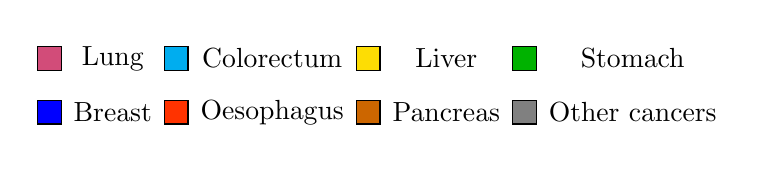
\begin{tikzpicture}
  \matrix [row sep=4pt, column sep=1pt] {
    \node[draw, fill=purple!70, minimum size=0.3cm] {}; & \node {Lung}; &
    \node[draw, fill=cyan, minimum size=0.3cm] {}; & \node {Colorectum}; &
    \node[draw, fill=yellow!80!orange, minimum size=0.3cm] {}; & \node {Liver}; &
    \node[draw, fill=green!70!black, minimum size=0.3cm] {}; & \node {Stomach}; \\
    
    \node[draw, fill=blue, minimum size=0.3cm] {}; & \node {Breast}; &
    \node[draw, fill=orange!40!red, minimum size=0.3cm] {}; & \node {Oesophagus}; &
    \node[draw, fill=orange!80!black, minimum size=0.3cm] {}; & \node {Pancreas}; &
    \node[draw, fill=gray, minimum size=0.3cm] {}; & \node {Other cancers}; \\
  };
\end{tikzpicture}

\caption{Estimated number of cancer-related deaths in 2020 across major cancer types, both sexes and all ages.}
\label{fig:new_deaths_2020}
\end{figure}









\section{Disucssion}

AI systems designed for cancer risk assessment and detection have become a vital subject of interest over the past few years. Research investigations confirm that AI applications will revolutionize how medical professionals detect cancer at its early stages. This study examines both the AI methodologies combined with datasets alongside the utilized AI approaches to show the improvements and remaining gaps in the research field. \cite{1} highlights in his work about guidelines, the critical need for early screening tests for prostate, colorectal, and endometrial cancers. AI-based early detection systems that process clinical information together with patient records, along with imaging output, and malignancy observations, before existing diagnostic processes. The recommendations from the American Cancer Society served as an essential starting point for subsequent research on AI screening technologies that focus on enhancing standard screening interfaces. Early oral cancer diagnosis remains a primary subject of investigation in the work presented by \cite{2}. Through his review, he demonstrates how artificial intelligence helps detect oral cancer at an early stage using both diagnostic and genetic information \cite{14}.


\subsection{Public Datasets and Benchmarks}

AI-based methods for risk assessment and early cancer screening have shown great potential for many cancer types. AI models are increasing the precision and effectiveness of cancer detection by utilizing a variety of data modalities, including imaging, genomics, and clinical data. Public datasets, which give researchers access to high-quality, real-world data, are now crucial for training and assessing these models. Even while these datasets have made incredible progress possible, issues with data integration, quality, and uniform review procedures still exist, impeding the broad clinical use of AI in oncology.


AI-based approaches to cancer risk evaluation, together with early disease detection, show extensive capabilities for numerous cancer types. AI detection methods have improved cancer diagnosis through their ability to process medical imaging along with genomics results and clinical information. The development of public databases containing research-grade data has become essential for both model training and assessment purposes.
Multiple important public datasets exist for use in cancer detection alongside risk prediction work.
Various studies make use of public datasets to build and verify AI models for breast cancer detection. The Digital Database for Screening Mammography (DDSM) serves as a leading dataset for mammography-based screening applications, together with its equivalent referenced in two and four. A public collection of breast cancer images needed for training deep learning algorithms includes the annotated mammography pictures. 
The development of AI models targeting lung cancer became robust thanks to the applications of imageomics. Medical researchers develop lung cancer screening models through image-based approaches by utilizing public information found in LIDC-IDRI, which provides CT scans with lung nodule annotations \cite{12}. Lung cancer genetic investigation and complete risk prediction through image-genomic data integration make use of TCGA together with additional genomic databases \cite{10}.


\subsection{Dataset Availability and Accessibility}
Researchers worldwide gain simple access to public datasets through open-access platforms, including Kaggle and GDC (Genomic Data Commons), and SEER and GEO \cite{5}. Illuminating cancer detection and risk analysis find their advancement through competitions organized by platforms like Kaggle, where academic scholars join forces to develop innovative strategies \cite{27}. These data platforms offer access to raw or processable datasets, which become available to users after clearance and a platform registration procedure \cite{25}. Data format standardization problems persist and prevent effective data sharing across different platform sources.
Research consortia, together with collaborative data-sharing platforms, eliminate barriers, which makes numerous datasets from different sources accessible to researchers \cite{4}. The TCGA project provides researchers with both genomic and transcriptomic information in addition to clinical data, while the SEER initiative gives detailed information about cancer incidence and survival numbers \cite{18}. These platforms enable international collaboration as well as diverse research tasks to ensure proper training of AI models through representative and extensive datasets.
The extensive availability of these databases has benefited AI research extensively, yet scientists must handle medical data access by studying both privacy concerns and ethical guidelines.
\subsection{Challenges with Public Datasets}
Worldwide research teams obtain access to public datasets through open-access platforms, which include Kaggle and GDC (Genomic Data Commons), and SEER and GEO. Illuminating cancer detection and risk analysis find their advancement through competitions organized by platforms like Kaggle, where academic scholars join forces to develop innovative strategies \cite{27}. These data platforms offer access to raw or processable datasets, which become available to users after clearance and a platform registration procedure \cite{25}. Data format standardization problems exist despite the fact that it becomes difficult to combine data from multiple sources.
Research consortia, together with collaborative data-sharing platforms, eliminate barriers, which makes numerous datasets from different sources accessible to researchers \cite{4}. The TCGA project provides researchers with both genomic and transcriptomic information in addition to clinical data, while the SEER initiative gives detailed information about cancer incidence and survival numbers \cite{18}. 
TInvestigators who use medical data need to ensure the protection of patient identity through anonymization, together with compliance with all relevant legal requirements, specifically including HIPAA and GDPR.

AI models used for cancer detection are assessed through AUC (Area Under the Curve), accuracy, sensitivity, and specificity measurements \cite{3}. AI model validation remains incomplete because existing metrics have different standards across datasets, which creates performance benchmarking gaps. The evaluation standards developed by SEER and Kaggle through their AI contests and benchmark competitions help researchers analyze cancer datasets relatively \cite{21}.  
Among all details used for AI model evaluation, cross-validation stands out as the most important technical implementation. The cross-validation method ensures that AI models receive robust training, which avoids specific data dependence.
\subsection{Benchmarks for Cancer AI Models}
AI models used for cancer detection are assessed through AUC (Area Under the Curve), accuracy, sensitivity, and specificity measurements \cite{3}. AI model validation remains incomplete because existing metrics have different standards across datasets, which creates performance benchmarking gaps. The evaluation standards developed by SEER and Kaggle through their AI contests and benchmark competitions help researchers analyze cancer datasets relatively \cite{21}. The cross-validation method ensures that AI models receive robust training, which avoids specific data dependence. Multiple partitions of the total dataset follow this technique to allow training models with specific partitions before validating them on different partitions for assessing their ability to produce generalizable outcomes in independent datasets.

\begin{comment}
\begin{figure}[htbp]
\centering
\begin{tikzpicture}
\begin{axis}[
    title={Accuracy vs. Study},
    ylabel={Accuracy},
    xlabel={Study},
    ymin=0, ymax=1.1,
    xtick=data,
    xticklabel style={rotate=45, anchor=east, font=\small},
    xticklabels={
        {Nie et al. 2020\\[21]},
        {Mokrane et al. 2020\\[22]},
        {Wang et al. 2019\\[23]},
        {Wu et al. 2019\\[24]},
        {Nie et al. 2021\\[25]}
    },
    ymajorgrids=true,
    grid style=dashed,
    width=0.48\textwidth,
    height=6.5cm,
    error bars/y dir=both,
    error bars/y explicit,
    scatter/classes={
        a={mark=*,blue}
    },
    every axis plot/.append style={blue, mark=*, mark options={fill=blue}, opacity=0.5}
]

\addplot+[
    only marks,
    error bars/.cd,
    y explicit,
]
coordinates {
    (0, 0.91) +- (0, 0.10)
    (1, 0.67) +- (0, 0.07)
    (2, 0.82) +- (0, 0.07)
    (3, 0.88) +- (0, 0.08)
    (4, 0.94) +- (0, 0.08)
};

\end{axis}
\end{tikzpicture}
\caption{Accuracy values from different studies with associated error bars representing uncertainty.}
\label{fig:accuracy_vs_study}
\end{figure} 
\end{comment}




\begin{table}[htbp]
\caption{Cancer Research Datasets Overview}
\centering
\begin{tabular}{|p{1cm}|p{1cm}|p{1cm}|p{1.5cm}|p{1.4cm}|}
\hline
\textbf{Dataset} & \textbf{Cancer Type(s)} & \textbf{Data Type(s)} & \textbf{Key Features} & \textbf{Accessibility} \\
\hline
TCGA \cite{1} & Breast, Lung, Colon & Genomic, Clinical, Transcriptomic & Gene expression, mutations, clinical data & GDC (Open Access) \\
\hline
Kaggle BC \cite{12} & Breast Cancer & Imaging, Clinical & Mammograms, patient history & Free on Kaggle \\
\hline
SEER \cite{13} & Multiple & Clinical, Epidemiological & Incidence, survival rates & SEER Website \\
\hline
Radiomics \cite{14} & Lung, Prostate, Breast & CT, MRI, Clinical & Tumor traits, lesion classification & Public access \\
\hline
GEO \cite{16} & Breast, Liver, Lung & Gene expression & RNA-Seq, microarray data & Open Access \\
\hline
\end{tabular}
\label{tab:cancer_datasets}
\end{table}




########
AI models successfully predicted cancer recurrence due to their capability to design proper postoperative strategies. Personalized medicine shows clear importance for prostate cancer treatment according to the studied outcomes, while AI technology provides methods to enhance treatment recommendation precision by personalized approaches. AI evaluation for early health system detection of epidemics and pandemics can be found in the literature . The main scope of this examination centered on AI disease prediction for infectious disease, but its findings extend equally to cancer research applications. 
 The recommendations from the American Cancer Society served as an essential starting point for subsequent research on AI screening technologies that focus on enhancing standard screening interfaces. Early oral cancer diagnosis remains a primary subject of investigation in the work presented by . Through his review, he demonstrates how artificial intelligence helps detect oral cancer at an early stage using both diagnostic and genetic information [14].AI evaluation for early health system detection of epidemics and pandemics can be found in the literature . The main scope of this examination centered on AI disease prediction for infectious diseases, but its findings extend equally to cancer research applications . 



The data collection regarding AI-based methods for cancer type identification can be found in Figure y.
Research presented  demonstrates that automated mammogram assessment through screening systems decreases human mistakes during analysis. The combination of AI-powered functions within breast cancer screening programs enables radiologists to detect detailed patients while improving their work process, which results in better patient outcomes alongside earlier medical diagnosis.
The ability of AI assessment for early cancer detection does not solve the basic problems regarding data enhancement standards and AI systems in healthcare delivery. More complete datasets need to feature diverse cancer profiles as well as demographic information about humans in a range of clinical instances. Standard quality standards in model evaluation improve the ability to compare diagnostic approaches and different cancer types in AI assessment systems.

\section{Conclusion}
Artificial intelligence has developed notable capabilities in early screening and risk prediction of cancer types such as lung cancer, breast cancer, prostate cancer, and oral cancers. AI models have been developed using genomic, clinical, and imaging data from various large data sources, including TCGA, LIDC-IDRI, SEER, and Kaggle Cancer Datasets. Innovative AI methods, such as support vector machines (SVMs), XGBoost, random forests, and convolutional neural nets (CNNs), have shown amazing improvements in the accuracy of diagnosis and early detection.
Some challenges still exist, with issues surrounding data quality, data imbalance, and the lack of a common standard for documenting models. In many studies, the generalizability of artificial intelligence models was limited, because of underrepresentation of the population differences, including diversity; interoperability of artificial intelligence models has also been hindered because of the differences in how datasets are formatted and the difficulty in comparing models as there are no standards for metrics to compare different models for the same purpose.
Going forward, it is essential that datasets are far more representative and inclusive, particularly those multimodal, incorporating imaging along with genetic and clinical data.
Artificial intelligence has the potential to make a significant difference in cancer screening by breaking through these barriers, in addition to allowing for the incorporation of every patient into a more individualized care protocol aimed at enhancing global patient outcomes.








\bibliographystyle{IEEEtran}
\bibliography{references}

\end{document}
